\section{Auswertung}
\subsection{Berechnung der Abklingdauer}
\label{sec:abklingdauer}
Die aufgenommenen Wertepaare aus Spannung $U(t)$ und $t$ wurden in \autoref{fig:bild1}
aufgetragen und es wurde eine Ausgleichsgrade der Form $f(x)=ax+b$ hindurchgelegt. Sie hat die Parameter:
\begin{center}
    $a=-30461.525 \pm 2711.401$\\
    $b=33.137 \pm 0.605$\\
\end{center}  
Aus der Steigung $a$ kann sofort über $T_{ex}=\frac{1}{2\pi \mu}=\frac{1}{a}$ die Abklingdauer berechnet werden. Sie liegt bei:
\begin{center}
    $T_{ex}=3.2828\times 10^{-5}$\\
\end{center}
\begin{figure}
    \centering
    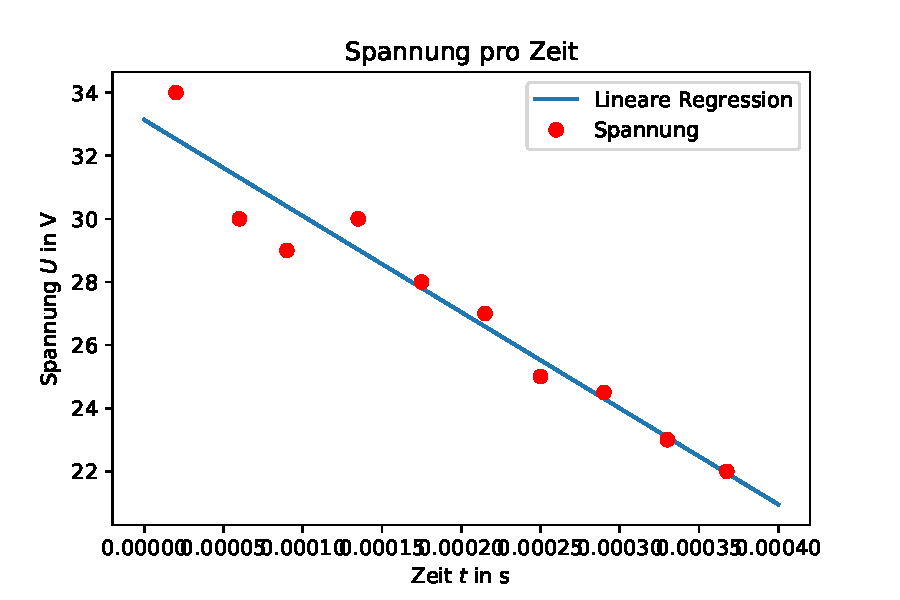
\includegraphics{spannungsverlauf.pdf}
    \caption{Spannungsverlauf in der Zeit}
    \label{fig:bild1}
  \end{figure}

  \subsection{Der Aperiodische Grezfall}
  Der Widerstand wurde solange verändert bis der Aperiodische Grenzfall eingetreten ist. Der zu diesem Zeitpunkt eingestellte Widerstand liegt bei:
  \begin{center}
      $R_{ap}=\SI[]{2.91}[]{k\Omega}$
  \end{center}